\section{Конструкторская часть}
\subsection{Взаимодействие клиента и мастер-сервера}
\subsubsection{Общая схема}
Основными компонентами в разрабатываемом протоколе являются клиент, мастер-сервер и медиасерверы. Сначала клиент устанавливает соединение с мастер-сервером, запрашивает у него список доступных для дальнейшего взаимодействия хостов.

Общая схема обмена сообщениями между клиентом и мастер-серверов представлена на рисунке \ref{image:general}. 

\begin{figure}[h!]
	\begin{center}
		{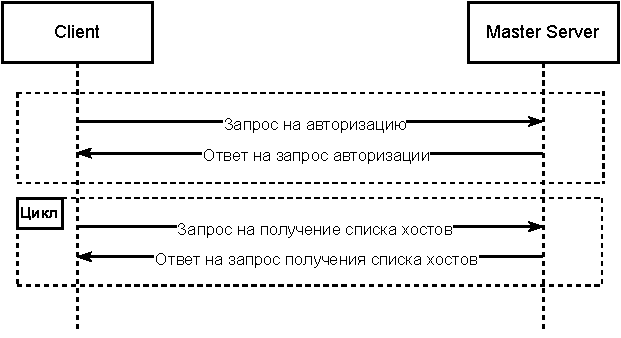
\includegraphics[scale = 1]{img/[general][master].pdf}}
		\caption{Общая схема.}
		\label{image:general}
	\end{center}
\end{figure}

\subsubsection{Авторизация}
Первый шаг в установке соединения между клиентом и мастер-сервером -- авторизация (рисунок \ref{image:auth}). 

\begin{figure}[h!]
	\begin{center}
		{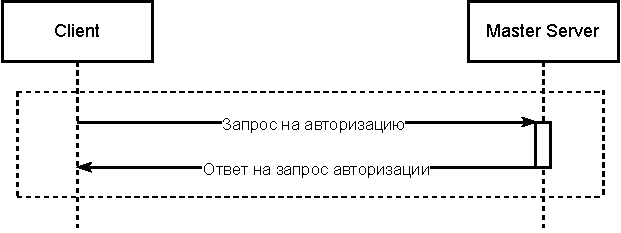
\includegraphics[scale = 1]{img/[items][master][auth].pdf}}
		\caption{Этап авторизации.}
		\label{image:auth}
	\end{center}
\end{figure}

Клиент отправляет авторизационный запрос в формате, представленном в таблице \ref{tbl:auth_request}.

\begin{longtable}{|p{4cm}|p{2cm}|p{9.5cm}|}
	\caption{Атрибутивный состав запроса на авторизацию}\label{tbl:auth_request}\\
	\hline
	
	\textbf{Параметр} & \textbf{Тип} & \textbf{Описание}\\ 
	\hline
	\endfirsthead
	
	\hline
	\textbf{Параметр} & \textbf{Тип} & \textbf{Описание}\\ 
	\hline
	\endhead
	
	\hline
	\multicolumn{3}{c}{\textit{Продолжение на следующей странице}}
	\endfoot
	\hline
	\endlastfoot
	
	username &
	string & 
	Имя пользователя доменной учетной записи \\
	
	\hline
	password & 
	string & 
	Пароль пользователя доменной учетной записи \\
	
	\hline
	grant\_type & 
	string & 
	Тип запроса на получение токена \\
	
	\hline
	client\_id & 
	string & 
	Имя приложения \\
\end{longtable} 

В зависимости от полученных данных сервер либо передаёт токен доступа в ответном сообщении (таблица \ref{tbl:auth_response_ok}), либо возвращает сообщение об ошибке авторизации (401 http-код) в формате из таблицы \ref{tbl:auth_response_err}.

\begin{longtable}{|p{4cm}|p{2cm}|p{9.5cm}|}
	\caption{Атрибутивный состав ответа на успешный запрос авторизации}\label{tbl:auth_response_ok}\\
	\hline
	
	\textbf{Параметр} & \textbf{Тип} & \textbf{Описание}\\ 
	\hline
	\endfirsthead
	
	\hline
	\textbf{Параметр} & \textbf{Тип} & \textbf{Описание}\\ 
	\hline
	\endhead
	
	\hline
	\multicolumn{3}{c}{\textit{Продолжение на следующей странице}}
	\endfoot
	\hline
	\endlastfoot
	
	access\_token &
	string & 
	Токен доступа \\
	
	\hline
	expires\_in & 
	integer & 
	Число миллисекунд, после которых токен перестанет быть валидным \\
	
	\hline
	token\_type & 
	string & 
	Тип токена \\
\end{longtable}

\begin{longtable}{|p{4cm}|p{2cm}|p{9.5cm}|}
	\caption{Атрибутивный состав ответа о непройденной авторизации на соответствующий запрос}\label{tbl:auth_response_err}\\
	\hline
	
	\textbf{Параметр} & \textbf{Тип} & \textbf{Описание}\\ 
	\hline
	\endfirsthead
	
	\hline
	\textbf{Параметр} & \textbf{Тип} & \textbf{Описание}\\ 
	\hline
	\endhead
	
	\hline
	\multicolumn{3}{c}{\textit{Продолжение на следующей странице}}
	\endfoot
	\hline
	\endlastfoot
	
	error &
	string & 
	Общее описание ошибки \\
	
	\hline
	error\_description & 
	string & 
	Детальное описание ошибки \\
\end{longtable}

\subsubsection{Получение списка хостов}
Далее в случае успешной авторизации клиент отправляет запрос на получение списка хостов (рисунок \ref{image:get_hosts_request}), к которым в последствии будут отправляться запросы на получение фрагментов видео.  

\begin{figure}[h!]
	\begin{center}
		{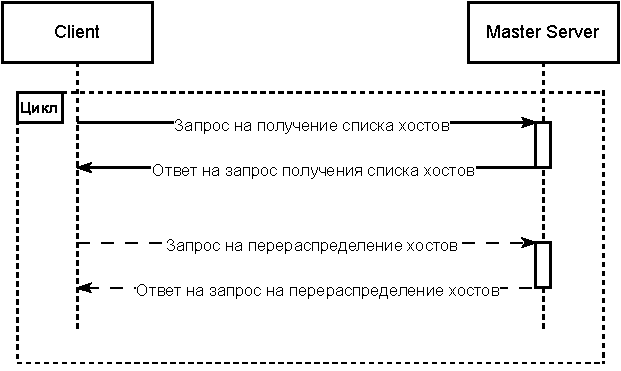
\includegraphics[scale = 1]{img/[items][master][share].pdf}}
		\caption{Этап получения списка хостов.}
		\label{image:get_hosts_request}
	\end{center}
\end{figure}

Формат такого запроса представлен в таблице \ref{tbl:get_hosts_request}, на рисунке \ref{image:get_hosts_request} обозначен как <<Запрос типа 1>>. 

\begin{longtable}{|p{4cm}|p{2cm}|p{9.5cm}|}
	\caption{Атрибутивный состав <<Запроса типа 1>>}\label{tbl:get_hosts_request}\\
	\hline
	
	\textbf{Параметр} & \textbf{Тип} & \textbf{Описание}\\ 
	\hline
	\endfirsthead
	
	\hline
	\textbf{Параметр} & \textbf{Тип} & \textbf{Описание}\\ 
	\hline
	\endhead
	
	\hline
	\multicolumn{3}{c}{\textit{Продолжение на следующей странице}}
	\endfoot
	\hline
	\endlastfoot
	
	access\_token &
	string & 
	Токен авторизации, указывается в заголовке запроса \\
	
	\hline
	video\_filename & 
	string & 
	Название видео-файла \\
	
	\hline
	start\_time & 
	timestamp & 
	Временная метка начала временного окна \\
	
	\hline
	end\_time & 
	timestamp & 
	Временная метка окончания временного окна \\
\end{longtable}

В ответ мастер-сервер отправляет список хостов с указанием диапазона кадров (<<Ответ типа 1>> на рисунке \ref{image:get_hosts_request}), которые можно с них загрузить, также дополнительно прилагается метаинформация о видеофайле (разрешение, длительность и т.д.). Атрибутивный состав этого сообщения приведён в таблице \ref{tbl:get_hosts_response}. 

\begin{longtable}{|p{4cm}|p{3cm}|p{8.5cm}|}
	\caption{Атрибутивный состав ответа на <<Запрос типа 1>>}\label{tbl:get_hosts_response}\\
	\hline
	
	\textbf{Параметр} & \textbf{Тип} & \textbf{Описание}\\ 
	\hline
	\endfirsthead
	
	\hline
	\textbf{Параметр} & \textbf{Тип} & \textbf{Описание}\\ 
	\hline
	\endhead
	
	\hline
	\multicolumn{3}{c}{\textit{Продолжение на следующей странице}}
	\endfoot
	\hline
	\endlastfoot
	
	hosts & 
	array[object] & 
	Список хостов с указанием адреса и диапазона кадров \\
	
	\hline
	\,\,\,\,\,\,\,address & 
	string & 
	Адрес хоста \\
	
	\hline
	\,\,\,\,\,\,\,frame\_start & 
	integer & 
	Номер первого фрагмента из диапазона \\
	
	\hline
	\,\,\,\,\,\,\,frame\_end & 
	integer & 
	Номер последнего фрагмента из диапазона \\
	
	\hline
	metadata & 
	object & 
	Блок метаданных \\
	
	\hline
	\,\,\,\,\,\,\,resolution & 
	string & 
	Разрешение \\
	
	\hline
	\,\,\,\,\,\,\,codec & 
	string & 
	Кодек \\
	
	\hline
	\,\,\,\,\,\,\,duration & 
	timestamp & 
	Длительность \\
\end{longtable}

Поскольку клиент запрашивает кадры видео только в пределах окна, то в случае его заполнения оно должно быть сдвинуто, и к мастер-серверу должен осуществляться повторный запрос на получение списка хостов (<<Запрос типа 1>>) для загрузки очередных фрагментов. Эта операция должна повторяться до тех пор, пока не будет получен весь видеофайл.

В случае, если клиенту не удаётся загрузить $n$ частей (значение этого параметра должно быть задано в конфигурационном файле) видеофрагмента от одного и тоже же медиа-сервера в пределах текущего окна, то он должен отправить на мастер-сервер <<Запрос типа 2>>, в котором указывается проблемный хост и временная метка последней успешно загруженной части видеофрагмента, загружаемого с данного медиа-сервера. Атрибутивный состав сообщения приведён в таблице \ref{tbl:complaint_request}.

\begin{longtable}{|p{4cm}|p{2cm}|p{9.5cm}|}
	\caption{Атрибутивный состав <<Запроса типа 2>>}\label{tbl:complaint_request}\\
	\hline
	
	\textbf{Параметр} & \textbf{Тип} & \textbf{Описание}\\ 
	\hline
	\endfirsthead
	
	\hline
	\textbf{Параметр} & \textbf{Тип} & \textbf{Описание}\\ 
	\hline
	\endhead
	
	\hline
	\multicolumn{3}{c}{\textit{Продолжение на следующей странице}}
	\endfoot
	\hline
	\endlastfoot
	
	access\_token &
	string & 
	Токен авторизации, указывается в заголовке запроса \\
	
	\hline
	video\_filename & 
	string & 
	Название видео-файла \\
	
	\hline
	start\_time & 
	timestamp & 
	Временная метка последней успешно загруженной части видеофрагмента \\
	
	\hline
	end\_time & 
	timestamp & 
	Временная метка окончания временного окна \\
\end{longtable}

Отправляя <<Запрос типа 2>> клиент инициирует повторную операцию определения подходящих для взаимодействия хостов. В ответ мастер-сервер отправляет новое перераспределение фрагментов видео между медиа-серверами, состав ответа приведён в таблице \ref{tbl:complaint_response}.

\begin{longtable}{|p{4cm}|p{3cm}|p{8.5cm}|}
	\caption{Атрибутивный состав ответа на <<Запрос типа 2>>}\label{tbl:complaint_response}\\
	\hline
	
	\textbf{Параметр} & \textbf{Тип} & \textbf{Описание}\\ 
	\hline
	\endfirsthead
	
	\hline
	\textbf{Параметр} & \textbf{Тип} & \textbf{Описание}\\ 
	\hline
	\endhead
	
	\hline
	\multicolumn{3}{c}{\textit{Продолжение на следующей странице}}
	\endfoot
	\hline
	\endlastfoot
	
	hosts & 
	array[object] & 
	Список хостов с указанием адреса и диапазона кадров \\
	
	\hline
	\,\,\,\,\,\,\,address & 
	string & 
	Адрес хоста \\
	
	\hline
	\,\,\,\,\,\,\,frame\_start & 
	integer & 
	Номер первого фрагмента из диапазона \\
	
	\hline
	\,\,\,\,\,\,\,frame\_end & 
	integer & 
	Номер последнего фрагмента из диапазона \\
	
	\hline
	metadata & 
	object & 
	Блок метаданных \\
	
	\hline
	\,\,\,\,\,\,\,resolution & 
	string & 
	Разрешение \\
	
	\hline
	\,\,\,\,\,\,\,codec & 
	string & 
	Кодек \\
	
	\hline
	\,\,\,\,\,\,\,duration & 
	timestamp & 
	Длительность \\
\end{longtable}

\subsubsection{Получение видеофрагментов}
Общая схема загрузки видеофрагмента показана на рисунке \ref{image:general_upload}. После получения списка доступных хостов от мастер-сервера клиент отправляет сразу несколько запросов на загрузку частей фрагмента параллельно. Таким образом, осуществляется одновременное скачивание сразу нескольких частей видео-файла в рамках текущего окна загрузки. 

\begin{figure}[h!]
	\begin{center}
		{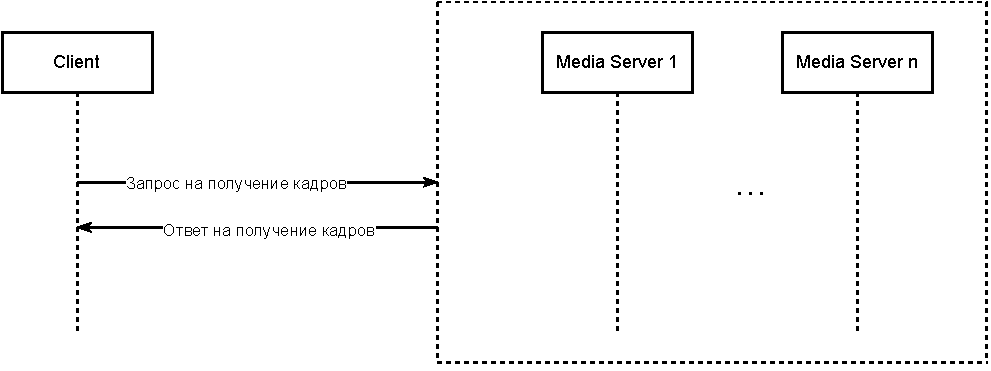
\includegraphics[scale = 1]{img/[general][media].pdf}}
		\caption{Общая схема получения видеофрагментов.}
		\label{image:general_upload}
	\end{center}
\end{figure}

На рисунке \ref{image:detailed_upload} представлена более детальная схема этого этапа. Параллельные запросы (<<Запрос типа 3>> таблица \ref{tbl:items_request}) к медиа-серверам будут осуществляться до тех пор, пока не будет получена большая часть окна загрузки, после чего оно динамически сдвигается, и клиент запрашивает у мастер-сервера список новых хостов. 

\begin{figure}[h!]
	\begin{center}
		{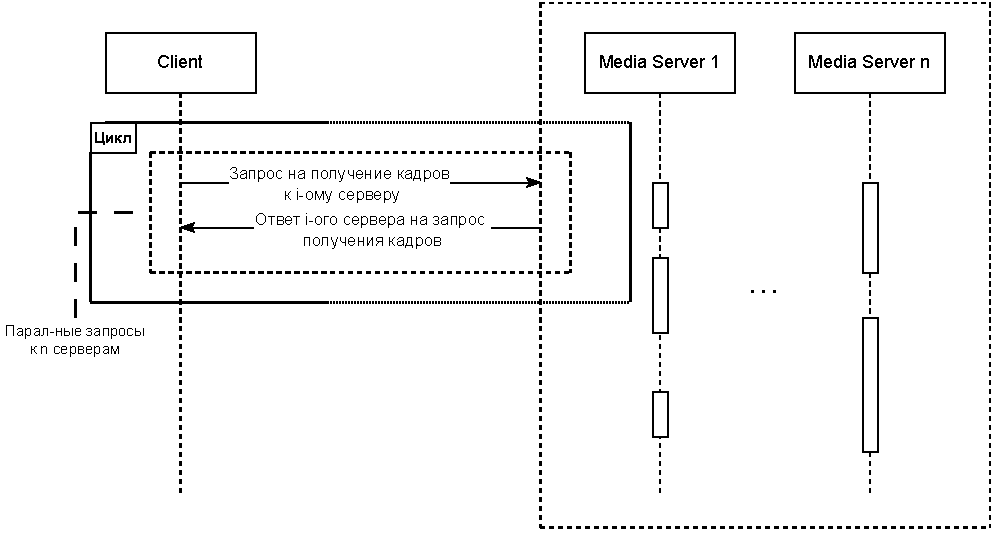
\includegraphics[scale = 1]{img/[items][media].pdf}}
		\caption{Установка соединения.}
		\label{image:detailed_upload}
	\end{center}
\end{figure}

\begin{longtable}{|p{4cm}|p{2cm}|p{9.5cm}|}
	\caption{Атрибутивный состав <<Запроса типа 3>>}\label{tbl:items_request}\\
	\hline
	
	\textbf{Параметр} & \textbf{Тип} & \textbf{Описание}\\ 
	\hline
	\endfirsthead
	
	\hline
	\textbf{Параметр} & \textbf{Тип} & \textbf{Описание}\\ 
	\hline
	\endhead
	
	\hline
	\multicolumn{3}{c}{\textit{Продолжение на следующей странице}}
	\endfoot
	\hline
	\endlastfoot
	
	access\_token &
	string & 
	Токен авторизации, указывается в заголовке запроса \\
	
	\hline
	video\_filename & 
	string & 
	Название видео-файла \\
	
	\hline
	frame\_start & 
	integer & 
	Номер первого фрагмента из диапазона \\
	
	\hline
	frame\_end & 
	integer & 
	Номер последнего фрагмента из диапазона \\
\end{longtable}

В ответ на поступивший запрос медиа-сервер формирует ответ, атрибутивный состав которого представлен в таблице \ref{tbl:items_response}.

\begin{longtable}{|p{4cm}|p{3cm}|p{8.5cm}|}
	\caption{Атрибутивный состав <<Запроса типа 3>>}\label{tbl:items_response}\\
	\hline
	
	\textbf{Параметр} & \textbf{Тип} & \textbf{Описание}\\ 
	\hline
	\endfirsthead
	
	\hline
	\textbf{Параметр} & \textbf{Тип} & \textbf{Описание}\\ 
	\hline
	\endhead
	
	\hline
	\multicolumn{3}{c}{\textit{Продолжение на следующей странице}}
	\endfoot
	\hline
	\endlastfoot
	
	num\_frames &
	integer & 
	Число передаваемых кадров \\
	
	\hline
	frames & 
	array[object] & 
	Список кадров \\
	
	\hline
	\,\,\,\,\,\,\,size & 
	integer & 
	Размер в байтах \\
	
	\hline
	\,\,\,\,\,\,\,frame & 
	array[byte] & 
	Кадр \\
\end{longtable}

\pagebreak